% Options for packages loaded elsewhere
\PassOptionsToPackage{unicode}{hyperref}
\PassOptionsToPackage{hyphens}{url}
%
\documentclass[
  12pt,
]{article}
\usepackage{amsmath,amssymb}
\usepackage{iftex}
\ifPDFTeX
  \usepackage[T1]{fontenc}
  \usepackage[utf8]{inputenc}
  \usepackage{textcomp} % provide euro and other symbols
\else % if luatex or xetex
  \usepackage{unicode-math} % this also loads fontspec
  \defaultfontfeatures{Scale=MatchLowercase}
  \defaultfontfeatures[\rmfamily]{Ligatures=TeX,Scale=1}
\fi
\usepackage{lmodern}
\ifPDFTeX\else
  % xetex/luatex font selection
\fi
% Use upquote if available, for straight quotes in verbatim environments
\IfFileExists{upquote.sty}{\usepackage{upquote}}{}
\IfFileExists{microtype.sty}{% use microtype if available
  \usepackage[]{microtype}
  \UseMicrotypeSet[protrusion]{basicmath} % disable protrusion for tt fonts
}{}
\makeatletter
\@ifundefined{KOMAClassName}{% if non-KOMA class
  \IfFileExists{parskip.sty}{%
    \usepackage{parskip}
  }{% else
    \setlength{\parindent}{0pt}
    \setlength{\parskip}{6pt plus 2pt minus 1pt}}
}{% if KOMA class
  \KOMAoptions{parskip=half}}
\makeatother
\usepackage{xcolor}
\usepackage[margin=1in,margin=1in]{geometry}
\usepackage{graphicx}
\makeatletter
\def\maxwidth{\ifdim\Gin@nat@width>\linewidth\linewidth\else\Gin@nat@width\fi}
\def\maxheight{\ifdim\Gin@nat@height>\textheight\textheight\else\Gin@nat@height\fi}
\makeatother
% Scale images if necessary, so that they will not overflow the page
% margins by default, and it is still possible to overwrite the defaults
% using explicit options in \includegraphics[width, height, ...]{}
\setkeys{Gin}{width=\maxwidth,height=\maxheight,keepaspectratio}
% Set default figure placement to htbp
\makeatletter
\def\fps@figure{htbp}
\makeatother
\setlength{\emergencystretch}{3em} % prevent overfull lines
\providecommand{\tightlist}{%
  \setlength{\itemsep}{0pt}\setlength{\parskip}{0pt}}
\setcounter{secnumdepth}{5}
\usepackage{geometry}
\usepackage{setspace}
\ifLuaTeX
  \usepackage{selnolig}  % disable illegal ligatures
\fi
\usepackage[]{natbib}
\bibliographystyle{plainnat}
\usepackage{bookmark}
\IfFileExists{xurl.sty}{\usepackage{xurl}}{} % add URL line breaks if available
\urlstyle{same}
\hypersetup{
  pdftitle={Data Analysis Report - GROUP 7},
  pdfauthor={Gary Ding, Rebecca Ives, Hwanho Kim, Nicholas Wunderlin},
  hidelinks,
  pdfcreator={LaTeX via pandoc}}

\title{Data Analysis Report - GROUP 7}
\author{Gary Ding, Rebecca Ives, Hwanho Kim, Nicholas Wunderlin}
\date{}

\begin{document}
\maketitle

{
\setcounter{tocdepth}{2}
\tableofcontents
}
\section{Abstraction}\label{abstraction}

~~~~This project explores what factors influence how often volcanoes
rate of eruption. We got our data for The Smithsonian Institute which
has one of the world's most comprehensive databases on volcanoes and
volcanic eruptions active within the last 100,000 years. We combined two
data sets from the database that included eruption records and volcanic
characteristics to look for patterns. Our main focus was on variable
tectonic settings, primary rock type, volcano type, region and
continuous factors such as longitude, latitude, elevation and the year
of the last eruption from each volcano. Through EDA we noticed certain
trends. Tectonic settings, volcano types and regions had more frequent
eruptions. Of the continuous variables, the year of the last eruption
had the strongest correlation with eruption count which was followed by
elevation. We also found a noticeable exponential relationship between
eruption count and the recency of eruptions, volcanoes that have erupted
more recently tend to have more recorded eruptions. Because our response
variable was count, we used Poisson regression to model eruption
frequency. After fitting the model, in the Diagnostic plots we noticed a
funnel-shaped pattern in the residuals plot and some deviation from
normality that hinted at some overdispersion in our data. We adjusted
this in our final model. We also saw that latitude and longitude
effectively captured regional geographical influence. In the end, we
found that when and where a volcano erupted, along with what type of
volcano it is and the tectonic settings are key predictors of eruption
frequency. These insights can support better risk assessments,
especially in identifying volcanoes that may be more active and
hazardous. Identifying these patterns can help communicate and help
policymakers be more prepared for volcanic threats.

\section{Introduction}\label{introduction}

~~~~Volcanoes are deadly and destructive natural disasters that occur
every year. While it is hard to fully estimate, one study reports that
volcanoes cause, on average, a billion dollars of property damage each
year . There have been eruptions that have caused one billion in damage
and another that has caused seven\citep{britannica2025}. This does not
take into account the lasting effects. Volcanic eruptions are something
that is hard to predict. The information surrounding volcanic eruptions
is not always accurate and complete because some of these volcanoes
predate human life \citep{smithsonian2023}. While they are hard to
predict, we are interested in looking at if there are factors that
potentially make a volcano have more frequent eruptions compared to
others.

\section{Data and Methods}\label{data-and-methods}

\subsection{Data}\label{data}

~~~~Our data comes from The Smithsonian Institution, which has the
world's most comprehensive database on volcanoes and volcanic eruptions
active within the last 100,000 years.

~~~~In particular, we examined two datasets, the volcano dataset and the
eruption dataset. The volcano dataset contains 958 volcanoes, each with
26 variables. The eruption dataset consists of 11,178 eruptions and 15
variables for each eruption.

\subsection{Data Cleaning}\label{data-cleaning}

~~~~From these initial 41 variables across two datasets, we eventually
cut down to eight variables that we would consider for our model. Among
these eight variables, there were four continuous predictors,
last\_eruption\_year, latitude, longitude, and elevation. The other four
variables were categorical: tectonic\_settings, major\_rock\_1,
primary\_volcano\_type, and region.

~~~~From the volcano dataset, we removed country and subregion as there
was already region, longitude, and latitude which took into account the
geographical location of the volcano. Further, country and subregion
were deemed too specific, with 89 unique countries and 91 unique
subregions. The evidence\_category variable was removed as it indicated
the type of evidence used to determine that the geological structure was
indeed a volcano, which does not make sense to include when predicting
eruptions. All major and minor rock types were removed except for
major\_rock\_1 as these columns were mostly NAs. Volcanoes with more
than one major rock or any minor rocks were uncommon. Finally, we did
not consider any of the variables measuring the population surrounding
the volcano area. Due to the sheer magnitude of the geological forces at
play during a volcanic eruption, it is very unreasonable to believe that
humans can influence a volcanic eruption \citep{layton2023}.

~~~~For the eruptions dataset, no variables were ultimately considered
for model selection. It did not make sense to use most of the variables
from an individual eruption event to predict the eruption frequency.
Columns indicating the starting and end times were removed for this
reason, as they did not pertain to the actual characteristics of the
volcano. Similar reasoning was applied to area\_of\_activity, which was
also a mostly NA column. Analogous to the evidence\_category column in
the volcano dataset, it did not make sense to include
evidence\_method\_dating. Latitude and longitude were omitted as they
both were a duplicate of volcano data. The one index we considered
potentially useful was the Volcano Explosivity Index (VEI)
\citep{wikipedia2025}. We considered gathering the average VEI for a
given volcano, however there were too many NAs in this column to
utilize.

~~~~So, the eruption dataset was used solely to gather our response
variable for our model, num\_eruptions (the number of eruptions for each
volcano). Each eruption in the eruption dataset had a volcano\_number
attached to it which identified which volcano that eruption was
associated with. By counting the number of appearances of each unique
volcano\_number found in the eruptions data, we could count the number
of eruptions for a given volcano, and merge that data into our volcano
dataset as our response variable.

~~~~Now that we had narrowed down our columns, the data underwent some
final cleaning. Some volcanoes had NA in their last eruption year as it
was unknown when they last erupted. These volcanoes were removed from
our dataset. We also needed to clean up the primary volcano type column,
which had duplicate types such as ``Stratovolcano'',
``Stratovolcano(es)'' and ``Stratovolcano?''. We considered these as one
singular volcano type.

~~~~Our final cleaned data contained 657 volcanoes and 11 columns. 8
columns were for our predictors, 1 column for our response, and 2
columns provided identifying information for the volcano
(volcano\_number and volcano\_name). There are 10 tectonic settings, 10
major rock types, 16 primary volcano types, and 19 regions.

\section{EDA}\label{eda}

~~~~Once our data was cleaned, and we narrowed down the variables we
wanted to consider, we started by creating a correlation matrix that was
produced for our four continuous variables, and the response (Figure
below).

\begin{center}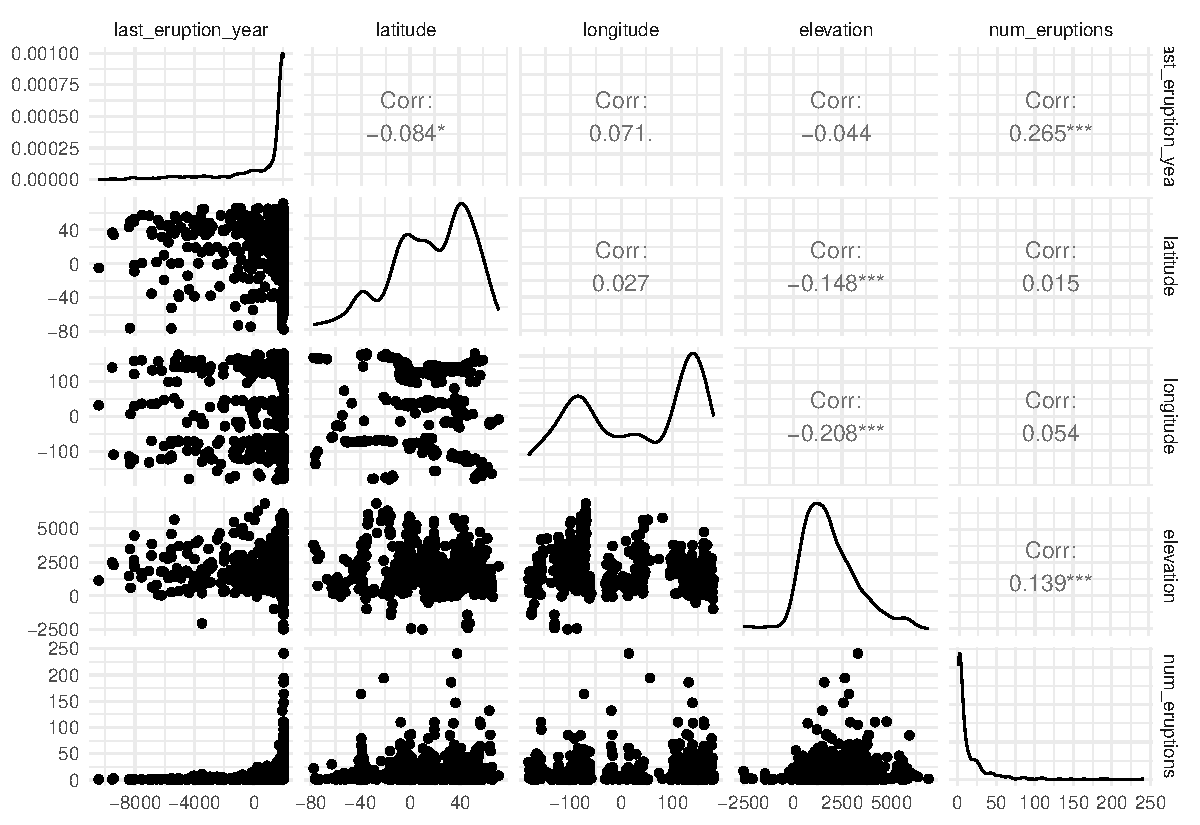
\includegraphics{Report_files/figure-latex/correlation-matrix-1} \end{center}

Based on the plots, it appears that most of the variables were not very
correlated with each other or with the response. There were a couple
plots that stood out though. First, elevation appeared to be at least
slightly positively correlated with our response (num\_eruptions). A
volcano's last eruption year appeared to have a very strong exponential
relationship with the response. This seems reasonable, as volcanoes that
erupt more frequently probably also have erupted more recently. Finally,
across the plots that include either latitude or longitude, there
appears to be some sort of clustering across the plots. This can be
observed most strongly with longitudes. This may be due to the fact the
volcanoes most commonly form along the edges of tectonic plates, leading
to the grouping in the data \citep{nps2022}.

Next, we created boxplots for the four categorical variables plotted
against the number of eruptions (the response), to investigate the
effects of different categories on. We made two iterations of these
plots. The first of these included the outliers, and is shown here.

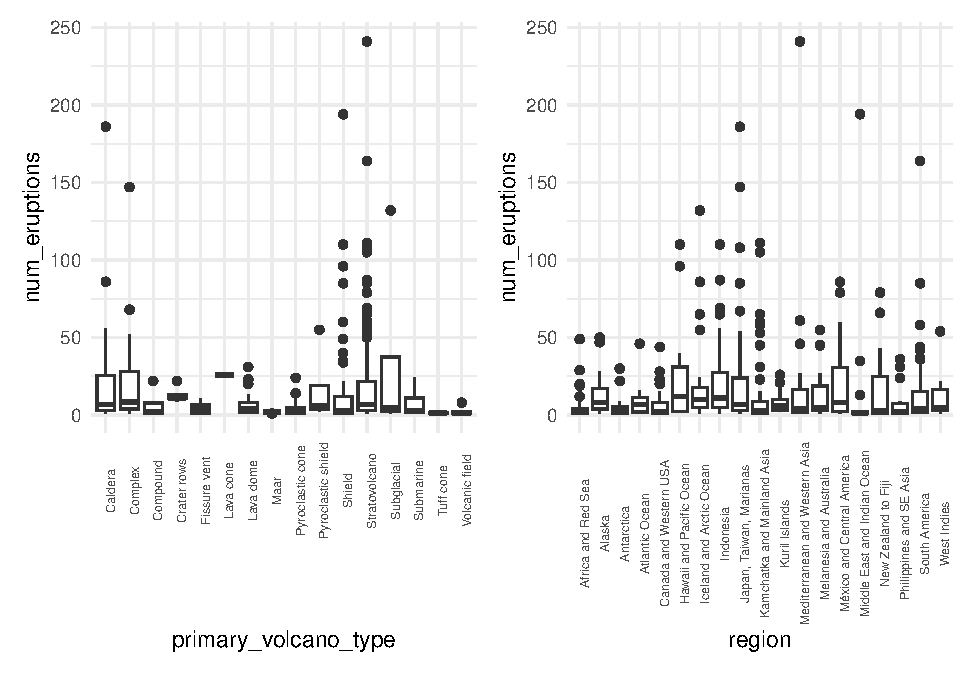
\includegraphics{Report_files/figure-latex/unnamed-chunk-1-1.pdf}
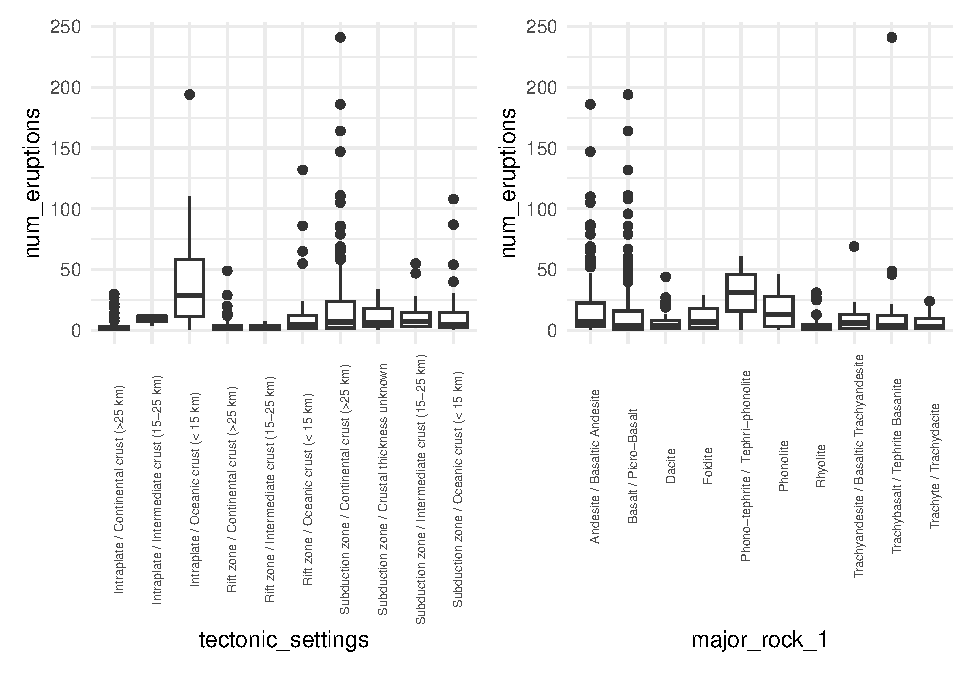
\includegraphics{Report_files/figure-latex/unnamed-chunk-1-2.pdf}

From these plots, it seems that there are quite a few outliers across
the dataset in general, and some categories have greater variance than
other categories. It also appears that the median values are mostly the
same for across a given category barring a few exceptions. Due to the
magnitude of the variance across the data, however, it was difficult to
distinguish the differences in median across categories. So, we also
plotted these categories while hiding the outliers in order to better
visualize the difference.
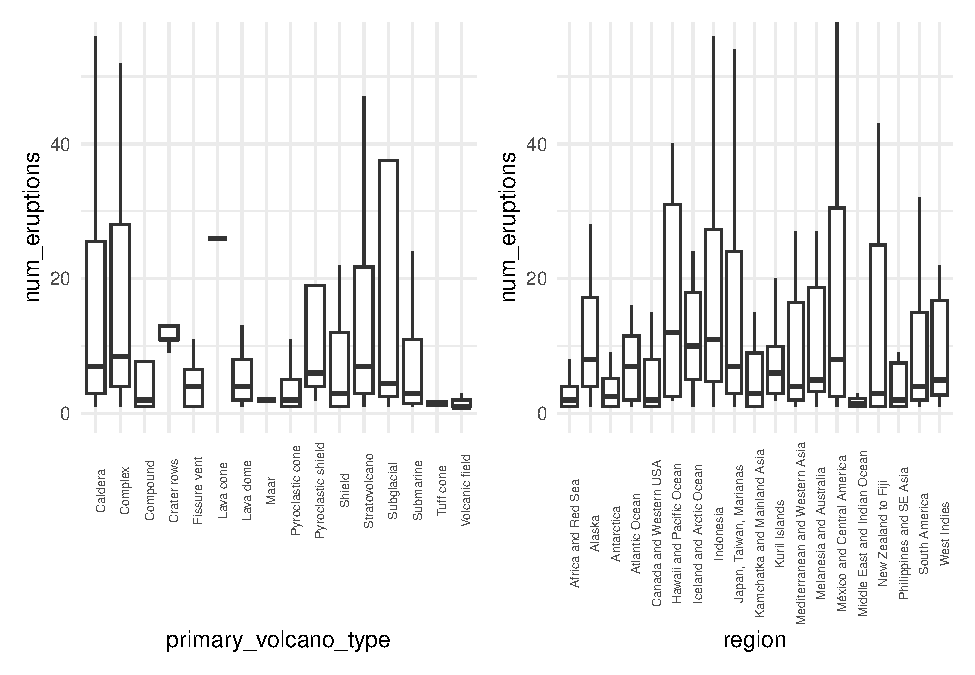
\includegraphics{Report_files/figure-latex/unnamed-chunk-2-1.pdf}
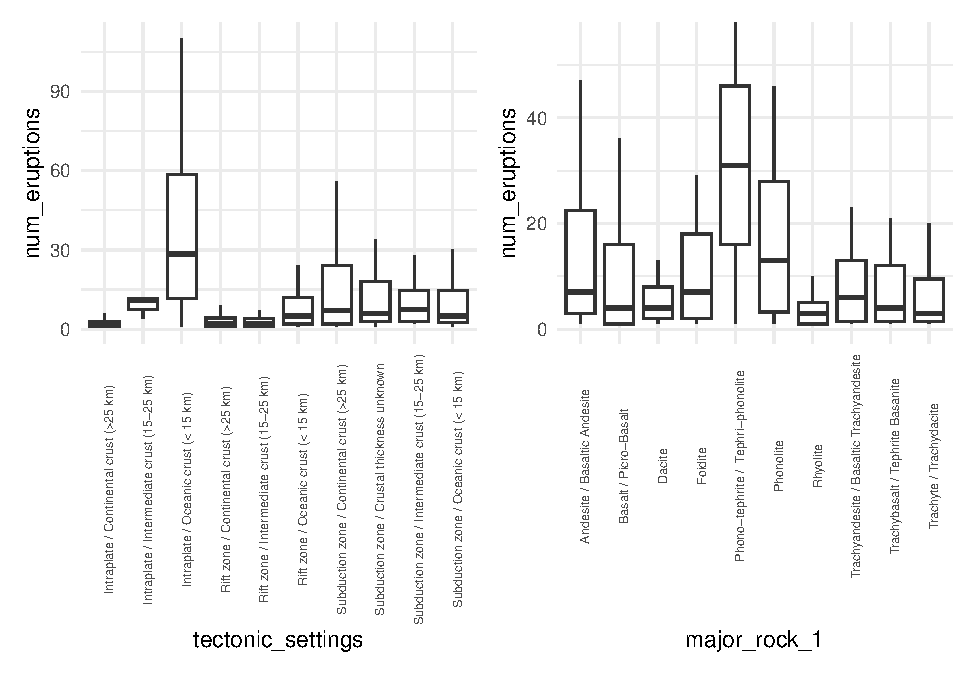
\includegraphics{Report_files/figure-latex/unnamed-chunk-2-2.pdf}

For Primary volcano type and Region, it is more difficult to tell which
categories are significant, or if any categories display some sort of
relationship with the response. However, the Intraplate / Oceanic Crust
(\textless15 km) category in tectonic settings and the Phono-tephrite /
Tephri-phonolite rock type in major\_rock\_1 seem to stand out as having
an effect on the response. This exploration will help us in our attempt
to simplify our categorical variables in our model.

Finally, though most geographical variables were removed during
cleaning, region as well as latitude in longitude were kept. We did take
note that these two variables were likely correlated. We investigated
this by plotting the boxplots showing the distribution of latitude and
longitude for a given region, ordered by increasing median, shown below.
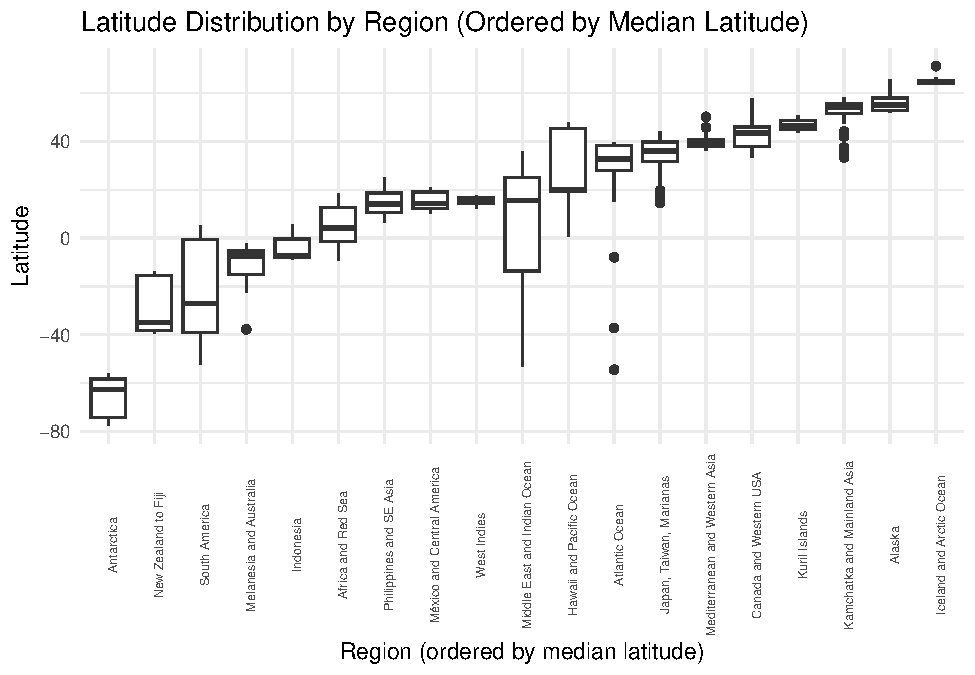
\includegraphics{Report_files/figure-latex/unnamed-chunk-3-1.pdf}
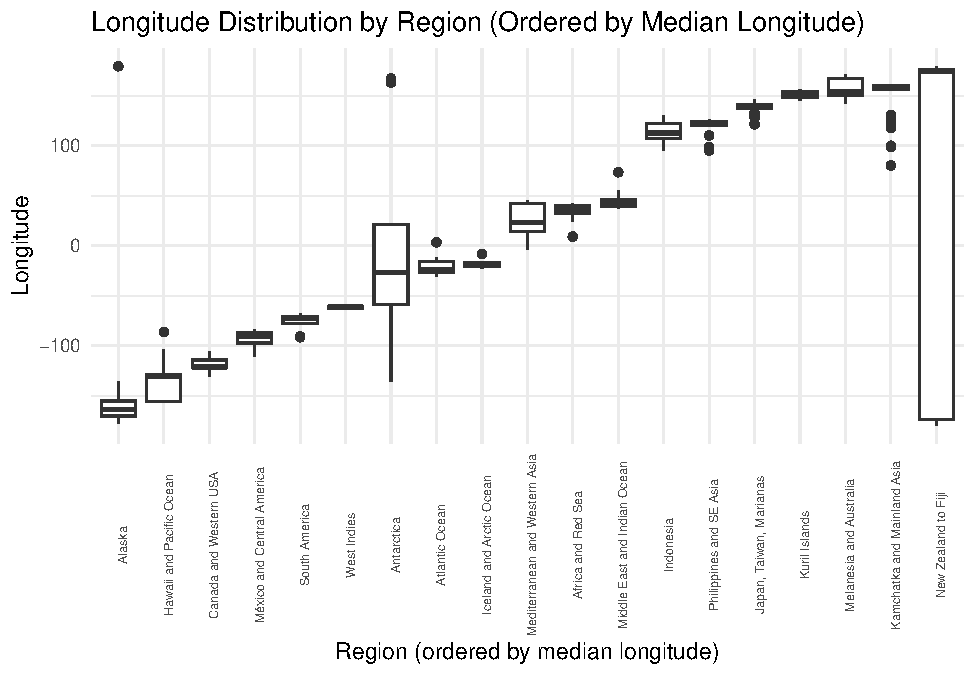
\includegraphics{Report_files/figure-latex/unnamed-chunk-3-2.pdf}

From these plots, it is quite clear that Region is a proxy for both
latitude and longitude. Generally, each region has a very small spread
of latitudes and longitudes, which makes sense, as they both refer to
the geographical location of a volcano. There is an interesting region
in the Longitude plot that is worth noting, in particular the far right
boxplot for New Zealand and Fiji has a giant spread that covers the
entire range of the data. This is actually due to the fact that New
Zealand and Fiji sit on the longitude line that transitions between -180
to +180. Beyond being an interesting result in our plot, this may be a
red flag for using longitude. 0 longitude is defined somewhat
arbitrarily, and if you go east far enough, you will end up west
eventually. So, how far east or west a volcano is might not be all that
meaningful. We keep all of this in mind during our model selection
process.

\section{Model}\label{model}

~~~~It was quickly identified that the Poisson model is the better
suited model for the data as it is looking at counts and rate of volcano
eruptions. In order to find the best model using the identified
variables, stepAIC was used. This allowed for it to be run both forwards
and backwards in order to find the best model. Eventually, it was found
that the best model for the data was the full model, consisting of all 8
of our predictors. We determined after investigating this model, that
our data was very overdispersed, however, it was decided that a simpler
model was desired, if possible. So, model selection continued based on
the poisson model, before converting our final model into a Quasi
Poisson model to account for the overdispersion.

~~~~Following the stepwise model selection, we wanted to look for ways
to simplify our model. As noted from our EDA, a region is a proxy to
latitude and longitude. As a result, we decided that our model should
contain both regions and either longitude or latitude. To determine
which one to keep, a series of ANOVA tests were performed to determine
which variables to keep. Specifically, we started with a model with all
the variables except region, longitude, and latitude. We found that, no
matter the order that we added region and longitude/latitude, the
addition of the variables all significantly improved the deviance of the
model. Unfortunately, not much was gained from this analysis. From here,
we compared the AIC and BIC of the models containing everything but
longitude and latitude against the model with everything but region. We
determined that both the AIC and BIC of the model with region instead of
longitude and latitude was better, so we elected to keep region over
latitude and longitude.

~~~~Building off of our EDA on our categorical variables, we attempted
to simplify our categories in the hopes that we could create a simpler
model by only examining factors that appeared impactful in our boxplots.
We tried selecting certain factors and creating an ``Other'' category
for the remaining categories that didn't exhibit a strong relationship
in our EDA, but such a model actually resulted in an increase in
deviance, fitting worse than the model with all the categories.

~~~~This leaves us with our final model:

\begin{align*}
\log(Y_i) =\ & \beta_0 \\
&+ \beta_1 \cdot \mathbb{I}(\text{PrimaryVolcanoType} = \text{Complex}) \\
&+ \beta_2 \cdot \mathbb{I}(\text{PrimaryVolcanoType} = \text{Compound}) \\
&+ \beta_3 \cdot \mathbb{I}(\text{PrimaryVolcanoType} = \text{Crater rows}) \\
&+ \beta_4 \cdot \mathbb{I}(\text{PrimaryVolcanoType} = \text{Fissure vent}) \\
&+ \beta_5 \cdot \mathbb{I}(\text{PrimaryVolcanoType} = \text{Lava cone}) \\
&+ \beta_6 \cdot \mathbb{I}(\text{PrimaryVolcanoType} = \text{Lava dome}) \\
&+ \beta_7 \cdot \mathbb{I}(\text{PrimaryVolcanoType} = \text{Maar}) \\
&+ \beta_8 \cdot \mathbb{I}(\text{PrimaryVolcanoType} = \text{Pyroclastic cone}) \\
&+ \beta_9 \cdot \mathbb{I}(\text{PrimaryVolcanoType} = \text{Pyroclastic shield}) \\
&+ \beta_{10} \cdot \mathbb{I}(\text{PrimaryVolcanoType} = \text{Shield}) \\
&+ \beta_{11} \cdot \mathbb{I}(\text{PrimaryVolcanoType} = \text{Stratovolcano}) \\
&+ \beta_{12} \cdot \mathbb{I}(\text{PrimaryVolcanoType} = \text{Subglacial}) \\
&+ \beta_{13} \cdot \mathbb{I}(\text{PrimaryVolcanoType} = \text{Submarine}) \\
&+ \beta_{14} \cdot \mathbb{I}(\text{PrimaryVolcanoType} = \text{Tuff cone}) \\
&+ \beta_{15} \cdot \mathbb{I}(\text{PrimaryVolcanoType} = \text{Volcanic field}) \\
&+ \beta_{16} \cdot \text{last\_eruption\_year} \\
&+ \beta_{17} \cdot \mathbb{I}(\text{Region} = \text{Alaska}) \\
&+ \beta_{18} \cdot \mathbb{I}(\text{Region} = \text{Antarctica}) \\
&+ \beta_{19} \cdot \mathbb{I}(\text{Region} = \text{Atlantic Ocean}) \\
&+ \cdots \\
&+ \beta_{53} \cdot \mathbb{I}(\text{MajorRock1} = \text{Trachyte / Trachydacite})
\end{align*}

The final model uses reference levels of Africa and Red Sea, Caldera,
Intraplate Continental, and Basalt/Picro-Basalalt. \(Y_i\) is a
realization from \(Y_i\) \textasciitilde{} Poisson(\(\lambda_i\)), for
i=1,\ldots..,n, where n=number of volcanos.

The final model still has noticeable limitations. One limitation is that
despite using a quasi-poisson model, the overdispersion for the data is
still quite high. This means that mean and variance are not quite equal
in this situation. However, to remain in the scope of this course, this
model was still our best option. To continue exploring this data set, it
could be worthwhile to investigate using a negative binomial model.
Another limitation is that AIC is not a viable option when using a
quasi-poisson model. While this was worked around to an extent by doing
Poisson and then fitting a quasi poisson, it could potentially lead to a
limitation. A more accurate option could have been to create all
different types of the model with different combinations of the variable
but using our method still creates a usable model. The final noticeable
limitation is that the model was formed as a retrospective study. Data
that has been collected over the years was used so there is not
necessarily a way to draw any causations from the model. However, it is
still beneficial to use as information and a way to plan for the future.

\section{Results}\label{results}

The results of the model show that there are several factors that
contribute to the number of potential eruptions. For example, the
volcano type Volcanic field has a significant decrease in your number of
eruptions while being a stratovolcanno increases the number of
eruptions. We also see a significant exponential relationship between
last eruption and eruption frequency. Volcanoes with more recent
activity demonstrate a lot higher eruption counts which make sense
because these volcanoes are early on in their ``active'' stage of their
volcanic life. We also found through our analysis that there is
substantial variability in our categorical variables. Tectonic Settings,
major rock types, primary volcano types and geographical regions
exhibited high eruption counts, specifically Subduction Zone, Andesite/
Basaltic Andesite, Stratovolcano and Japan, Alaska and Iceland for their
respective categorical variables that they are associated with. They all
specifically showed higher eruption counts than different categories in
their variable category.

According to our model, if everything is kept at its reference level but
years since last eruption is increased by 100, the confidence interval
at 95\% of the percentage increase in number of eruptions is 4.23\% and
7.645\%. If everything remains constant but elevation is increased by
1000 feet, the percentage increase in the number of eruptions, with a
95\% confidence interval, between 12.8\% and 38.3\%. So increasing the
elevation can have a large impact on the number of eruptions. Finally,
if everything remains constant but the region goes from Africa and Red
Sea to Alaska, the 95\% confidence interval is quite wide from a
34.941\% increase to a 325\% increase.

Since the model is the full model, it is no surprise that the residual
plots look pretty good. For the fitted versus residual, the points are
fairly randomly distributed. There is some clumping at the beginning but
that is a result of this data set being zero-bounded, as it is not
possible to have less than zero eruptions. The Q-Q plot of residuals
shows some tailing off towards the higher quantities of the plot which
is suggesting that our count data does show some overdispersion which is
a common challenge when modeling something like volcanic eruptions
because they are on the rare side. Overall, the diagnostic plots
performed well, which to us, was no surprise because our model was the
full model.

\section{Conclusion}\label{conclusion}

The overall conclusion is that there are a wide variety of factors that
go into the number of eruptions. It is important to look at its region,
rock type, last year's eruption, and other factors. Governments who have
volcanoes in their country that have factors that could potentially lead
to more eruptions should take necessary action to help their country
recover. They should look into potentially setting up a perimeter so
that people are not allowed to live inside. They should make sure to
have adequate funding to support their communities should a disaster
strike. The model can give governments a rough idea of their potential
risk factor so that they can plan accordingly.

For next steps with this data, as mentioned above, it is worthwhile
potentially exploring other models that may better address the
overdispersion that was noticed. It is also possible that looking at
some of the variables removed, such as minor rock types, could help make
the model more precise. As time goes on, tracking of this information
may get better allowing for the model to continue to improve.

\renewcommand\refname{References}
  \bibliography{references.bib}

\end{document}
